\documentclass[%
 aip,
amsmath,amssymb,
reprint,
]{revtex4-1}

\usepackage{graphicx}% Include figure files
\usepackage{dcolumn}% Align table columns on decimal point
\usepackage{bm}% bold math
\usepackage{verbatim}
\usepackage{subcaption}
%\usepackage[mathlines]{lineno}% Enable numbering of text and display math
%\linenumbers\relax % Commence numbering lines

\usepackage[utf8]{inputenc}
\usepackage[T1]{fontenc}
\usepackage{mathptmx}
\usepackage{etoolbox}
\usepackage{lipsum}


%% Apr 2021: AIP requests that the corresponding 
%% email to be moved after the affiliations
\makeatletter
\def\@email#1#2{%
 \endgroup
 \patchcmd{\titleblock@produce}
  {\frontmatter@RRAPformat}
  {\frontmatter@RRAPformat{\produce@RRAP{*#1\href{mailto:#2}{#2}}}\frontmatter@RRAPformat}
  {}{}
}%
\makeatother
\begin{document}

\preprint{AIP/123-QED}

\title[Intermediate Physics Laboratory 2, Module 2]{title}
% Force line breaks with \\
\author{Myeong-gi Jo}
\altaffiliation{
whaudrl4005@gmail.com
}
\author{Subin Kim}
\altaffiliation{
subini0213@snu.ac.kr
}
\author{Jeong Min Lee}
\altaffiliation{
jmleeluck@snu.ac.kr
}
\author{Eugene Park}
\altaffiliation{
eupark@snu.ac.kr
}
\affiliation{ 
Department of Physics and Astronomy, Seoul National University
}

\date{\today}
\begin{abstract}
this is abstract
\end{abstract}

\maketitle

\section{\label{sec:Intro} Introduction} 

Despite the common rule of analysis in electrical engineering being `linearization', most electrical phenomena should be explained in terms of non--linear electrical components. Op--Amp(Operation Amplifier) is one of the typical non--linear components. An important property of Op-Amp is that it saturates. Saturation occurs when the output voltage of the Op-Amp reaches its maximum or minimum limit and cannot increase or decrease any further. In the case of inverting Op--Amp, this leads to sudden positive feedback after a saturation point. Thus it is motivating to design non--linear resistor using inverting Op-Amp.

Another interesting non--component is MOSFET(Metal Oxide Semiconductor Field Effect Transistor). Unlike pnp or npn transistor, MOSFET has only one type of carrier which makes it much easier to control terminals for operation. Operation of MOSFET has three regions characterized by Gate--Source voltage($V_{\textrm{GS}}$) and Drain--Source voltage($V_{\textrm{DS}}$) as

\begin{itemize}
    \item Cut-off region ($V_{\textrm{GS}}<V_{\textrm{th}}$): MOSFET will be closed, and there will be no current flow through it. 
    \item Saturation region ($V_{\textrm{GS}}>V_{\textrm{th}}$, $V_{\textrm{DS}}>(V_{\textrm{GS}}-V_{\textrm{th}})$): Current across the drain to source terminal will remain almost constant despite the increment voltage across the drain to source.
    \item Linear region ($V_{\textrm{GS}}>V_{\textrm{th}}$, $V_{\textrm{DS}}<(V_{\textrm{GS}}-V_{\textrm{th}})$): Current across the drain to source terminal will linearly increase with the increment voltage across the drain to source.
\end{itemize}

\noindent where $V_{\textrm{th}}$ is threshold voltage. Thus MOSFET behaviors like a resistor in linear region. By short-circuiting the gate and source terminal, we can use MOSFET as a resistor that turns on after threshold voltage. Combining with Op--Amp, it gives additional discontinuos slope to the $I-V$ curve.

This report is organized as follows. In section II, we introduce our experimental method for designing and analyzing a non--linear resistor. In section III, we analyze the measurement data, the $I-V$ curve mainly. This includes the discussion of a discrepancy between measurement and theory, the effect of Op--Amp supply voltage, and hysteresis. We will summarize the whole arguments in section IV as a conclusion.

\section{\label{sec:Method} Method}

An ADTL082J was used as the Op-Amp, and IRF1010E was used for the n-channel MOSFETs. Before the experimental process, the $I-V$ characteristics of the MOSFETs were measured to obtain a threshold voltage and the effective resistance when the MOSFET was open, with the circuit as in FIG. \ref{MOSFET_circuitfig}. The output voltage of the Op-Amp was also measured to compensate for the saturation effects of the real--world Op--Amp. The negative resistor was designed with and without MOSFETs, and was measured with the circuit as in FIG. \ref{fig:Fig1} (a)(b), and the current was measured via a resistor in series in the negative resistor($R$). We sourced voltage from -5.0V to +5.0V in increments of 0.1V, and then in reversed order. We repeated the measurement for $R=10\>\Omega,\>47\>\Omega,\>220\>\Omega,\>560\>\Omega$.

As we will see later, the $I-V$ curve of the non--linear resistor can be divided into three regions with two distinguishable slopes and boundary points. We compared measured slopes and boundary points with theoretically calculated ones and then analyzed the discrepancy. We also explored how the range of the negative resistance region is changed when we differ Op-Amp supply voltage from 0V to 5V by 1V. Finally, we confirmed hysteresis, the difference between $I-V$ curves measured by increasing and decreasing voltage.

From resulting $I-V$ curve, we found boundary points and divided region by detecting extremum maximum or minimum points of $I-V$ curve. This is done by choosing maximum or minimum point on data array rather than regression of the graph near extremum points. There are a few cases that do not have extremum point, but have points which are a boundary of two regions with significantly different slopes. We directly selected boundary points at those cases.

As we divided regions, we linearly regressed each area. At circuit with MOSFETs such as FIG. \ref{fig:Fig1} (d), the slope continuously changes for short region, so we excluded such region for linear regression.


\section{\label{sec:Result} Result}

\subsection{Negative Resistance}
\begin{figure}[!h]
  \centering
  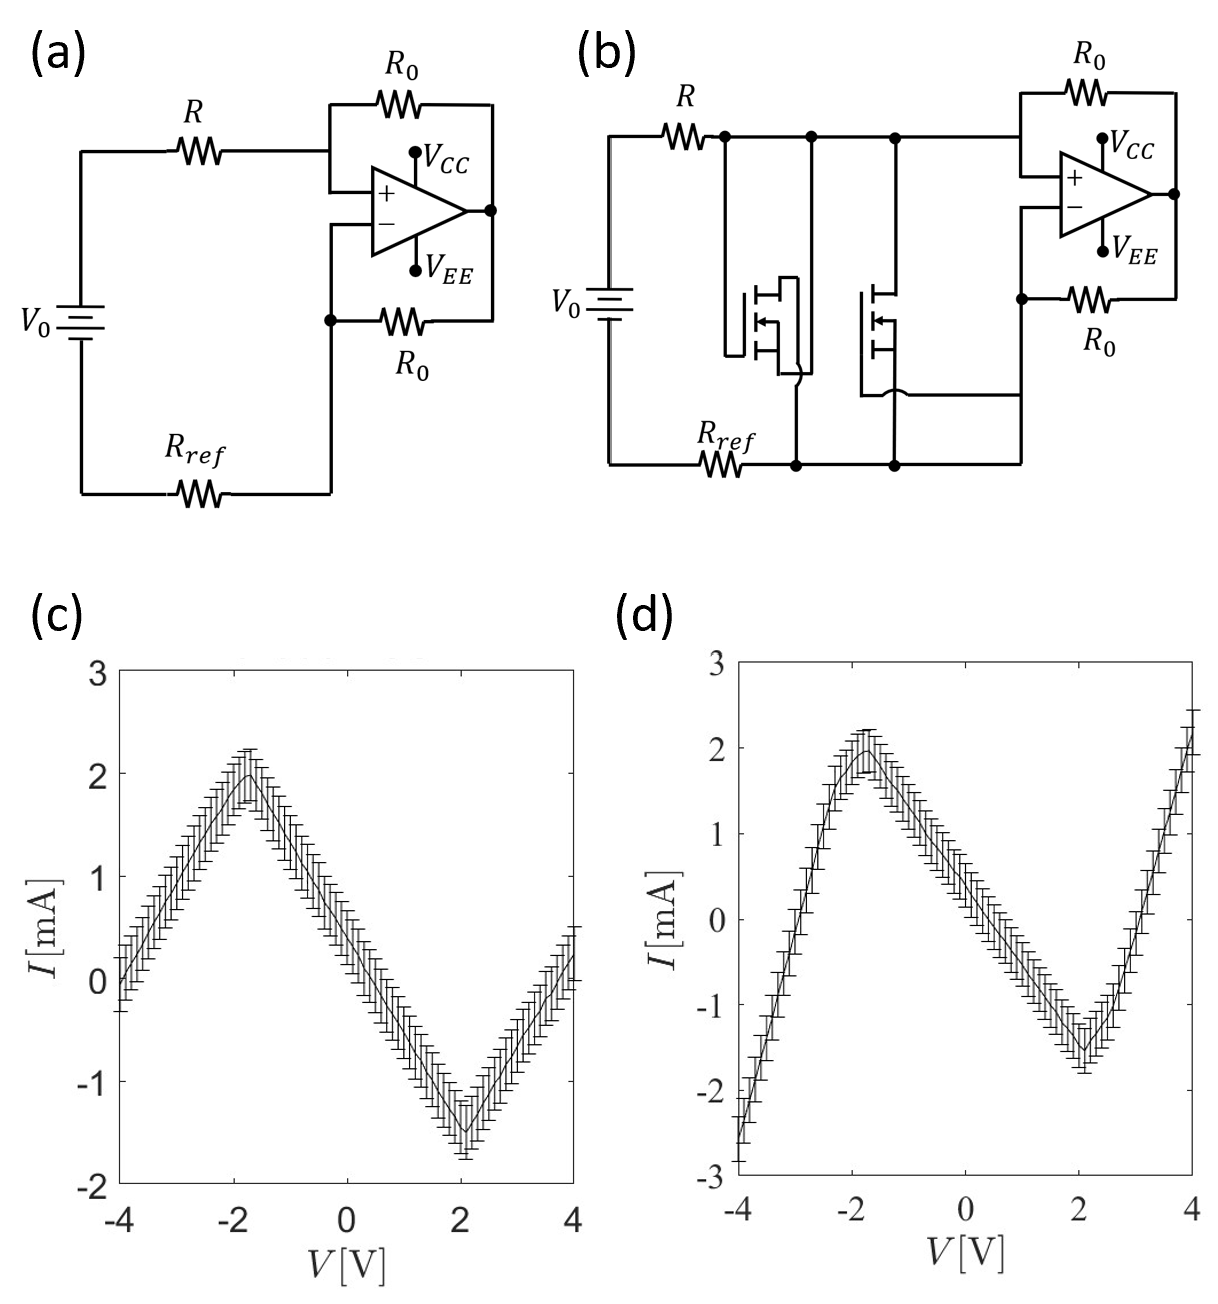
\includegraphics[width=0.45\textwidth]{figures/Fig1.png}
  \caption{$R = 47\Omega, R_{ref} = 1120\Omega, R_0 = 1k\Omega$. (a) schematic of circuit withot MOSFETs (b) schematic of circuit with MOSFETs (c) result of circuit without MOSFETs (d) result of circuit with MOSFETs}
  \label{fig:Fig1}
\end{figure}

%%$\textrm{R} = 47\Omega$, and $ \textrm{R_{ref}} = 1120\Omega $ $\textrm{R_0} = 1k\Omega$
Fig. \ref{fig:Fig1} (a) is a schematic of well known Op-Amp negative converter, and (b) is circuit of negative converter and MOSFETs, parallel connected. Total current of the circuit was experimented from -4V to 4V, and Fig. \ref{fig:Fig1} (c) and (d) is resulting current of given  input voltage. 


On region 1, we successively observed negative converter effect of Op-Amp. Current is negative while volage across the circuit is positive, and vice versa. On region 2, the slope gets positive rapidly because saturation occurs on this region. As the output is saturated, the output voltage does not changes, and the system allows voltage difference applied on Op-Amp. This results to invalidation of negative converting effect.

Effect of MOSFETs of region 1 is little, while positive slope is bigger on the circuit with MOSFETs on region 2. This is because at region 2 of circuit with MOSFETs, the voltage across the MOSFETs exceeds its threshold so that MOSFETs are activated, works like small resistance. This increases total flow of circuit so that the slope is bigger than that without MOSFETs. Between region 2 and extremum maxumum point of FIG. \ref{fig:Fig1} (d) with a continuous derivitive is the region with saturation, but not activated MOSFETs.




\subsection{Tuning Differential Resistance Slopes}
The slope of the negative differential region and the positive region, including the extreme points($V_\text{in}^0$) of the $I-V$ characteristics are shown in FIG. \ref{fig:Fig2}.

\begin{figure}[!h]
  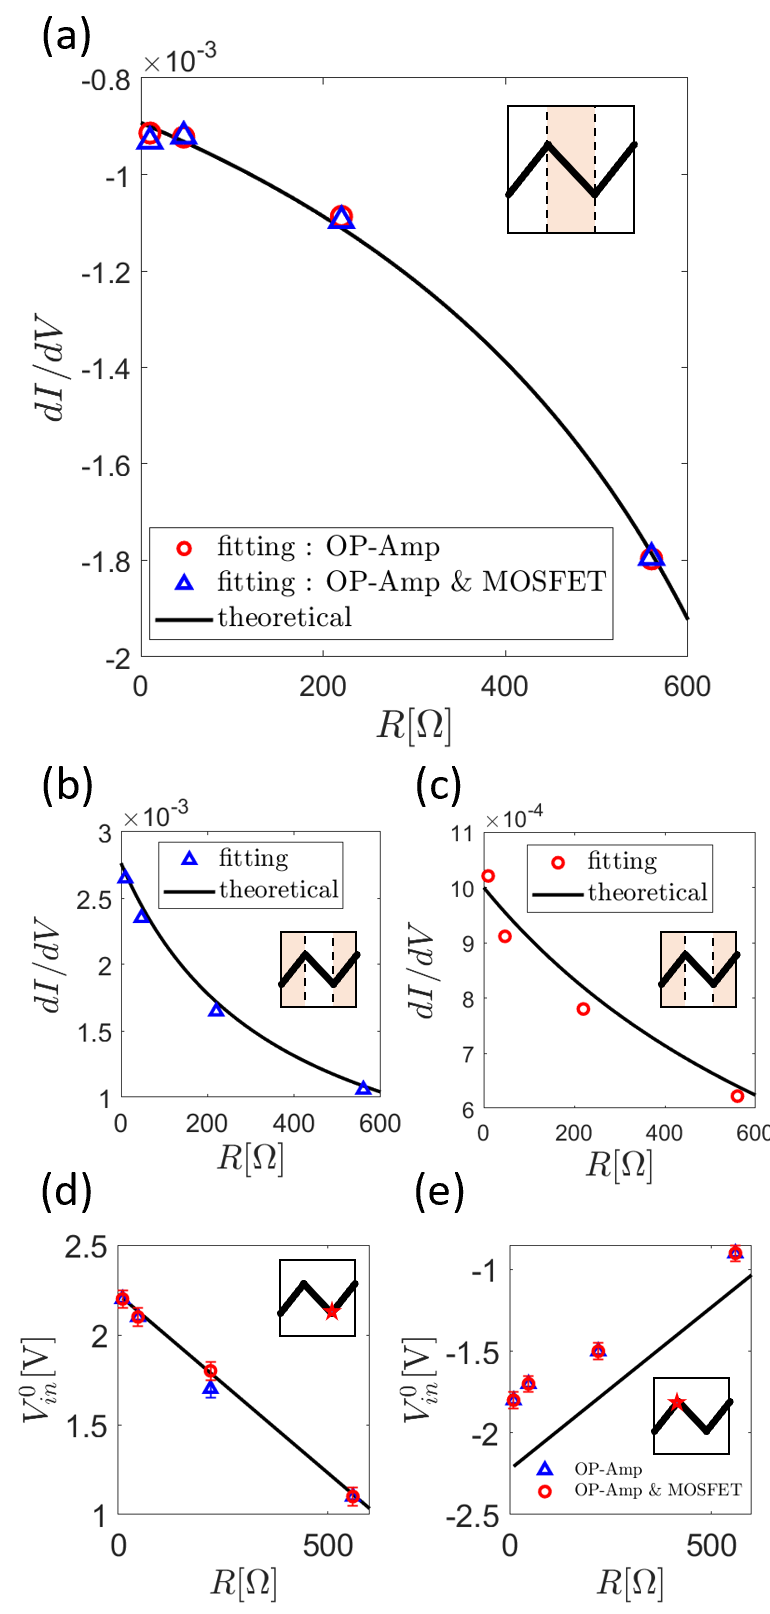
\includegraphics[width=0.45\textwidth]{figures/Fig2.png}
  \caption{The differential resistance of (a) region I, (b) region II for the Op-Amp and MOSFET negative resistor, (c) region II for the Op-Amp negative resistor, and the extreme points($V_\text{in}^{0}$) of both negative resistors having a (d) positive and (e) negative voltage value. The shaded region in the insets depict the fitted region, and the red stars indicate the extreme value position relative to the $I-V$ curve. A Op-Amp supply voltage of $5$V was used.}
  \label{fig:Fig2}
\end{figure}

As can be seen, region I (FIG.\ref{fig:Fig2}. (a)) does not differ by the addition of MOSFETs, and matches the theory well for both negative resistors. For region II, (FIG.\ref{fig:Fig2}. (b, c)) the MOSFETs nearly double the slope. Both cases match the theory well. The extreme points($V_\text{in}^0$) show a linear dependence, for both cases. The positive extreme points(FIG.\ref{fig:Fig2}. (d)) match the theory while the negative extreme points show a positive voltage shift(FIG.\ref{fig:Fig2}. (e)). We note that this discrepancy stems from the fact that the operating saturation voltage of the Op-Amp ADTL082J is not symmetrical, thus experimentally observed that the saturation occurs $\sim-3.5$V. This pushes the negative extreme points closer to $0$V. Despite this effect, the point for $V_0=0$ exhibits a negligible current flow $I\sim0.1$mA, excluding an unintended Op-Amp offset voltage as a possibility. \\

The higher slope of region II is due to the fact that the MOSFETs, acting as voltage gates, add another 'venting' channel for the current. Intuitively, the MOSFET effective resistor is smaller than $R_0$, thus decreasing the total resistance of the flowing current. The opposite effect can be obtained by adding high resistance resistors in series to each MOSFET and increasing the resistance of the flowing , thus decreasing the slope. Additionally, region I is indifferent to MOSFET addition since current does not flow through MOSFETs in this region. By changing a single resistor of the negative resistor proposed, various values of negative differential resistance can be obtained and theoretically predicted with out model. 

\subsection{Effect of Op-Amp Supply Voltage}
\begin{figure}[!h]
  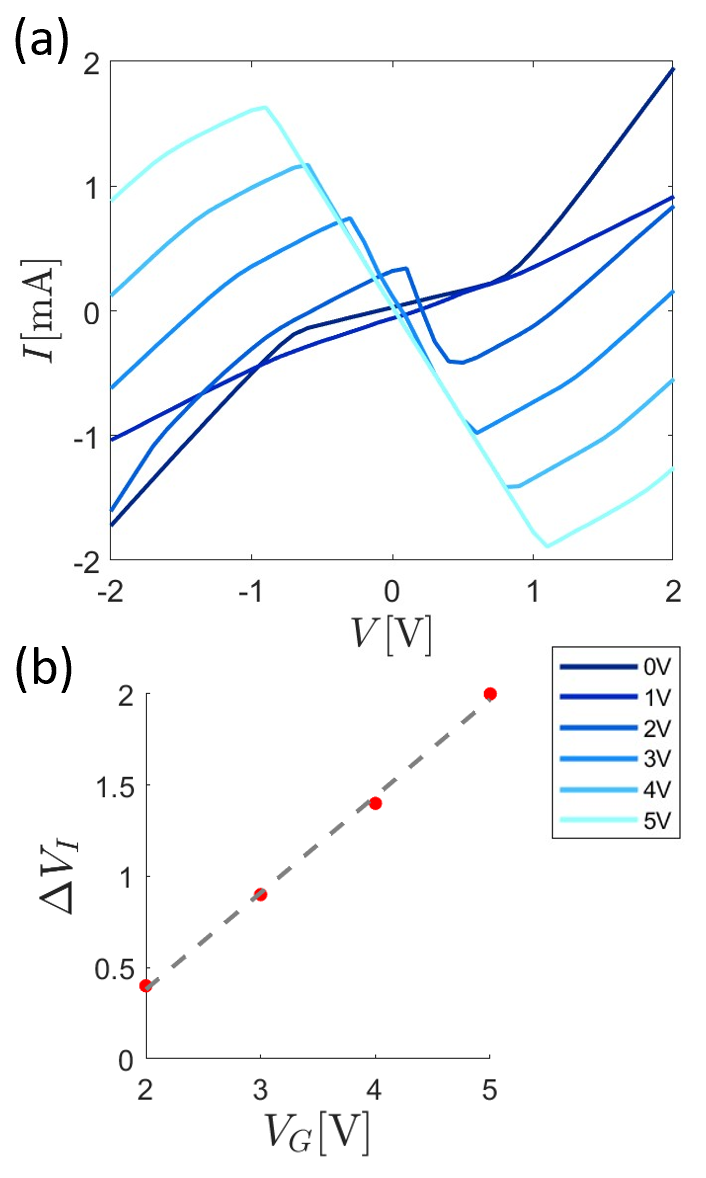
\includegraphics[width=0.45\textwidth]{figures/Fig3.png}
  \caption{(a) The $I-V$ curve varying by different supply voltage($V_G$).(b) the region of negative resistance for different $V_G$ with the linear regression. $R^2$ of this regression is 0.9979.}
  \label{fig:Fig3}
\end{figure}

By varying the supply voltage of OP-AMP, the region showing the negative resistance is getting broader. This can be verified it by seeing FIG. \ref{fig:Fig3} (a). For 0V and 1V, supply voltage is too small for negative resistance to appear. For the supply voltage greater or equal to 2V, the negative resistance starts to appear. We estimated the interval of negative resistance $\Delta V_I$ by subtracting two extreme points. If you see the FIG.\ref{fig:Fig3} (b), that region is strongly linear to the supply voltage. 

This linearity can be expected referring to the features of Op-Amp.
For ideal Op-Amp, $V_{\text{sat}} = V_G$. Even though the Op-Amp what we used in this experiment is not ideal, but still $V_{sat} \propto V_G$ since the deviation of real Op-Amp is not that significant in our experimental scale. Thus, by noting that the extreme point of each $I-V$ curve is moment that Op-Amp becomes saturated, $V_G \propto \Delta V_I$. This characteristic allows us to manage how much the area of negative resistance is appeared.


\subsection{Hysteresis Region}
\begin{figure}[!h]
  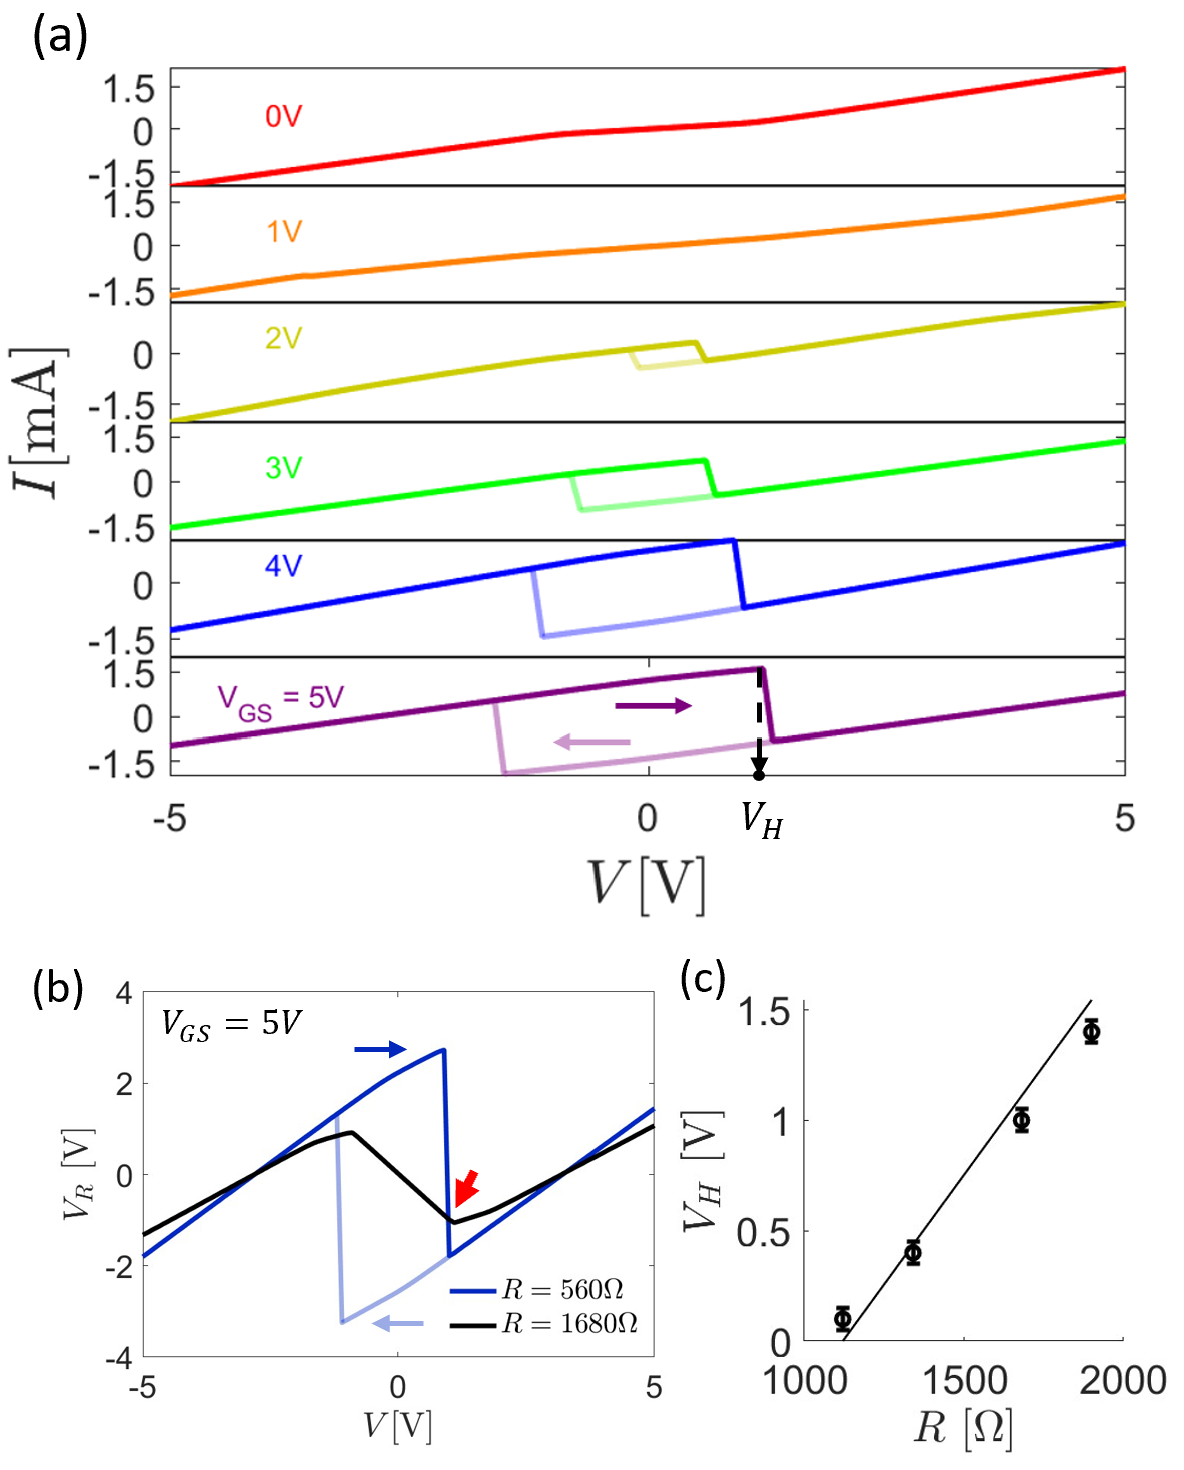
\includegraphics[width=0.48\textwidth]{figures/Fig4.png}
  \caption{(a) The $I-V$ curve of the negative resistor with Op-Amp and MOSFETs varying by different the supply voltage($V_{G}$). Hysterisis drop voltage $V_H$ is depicted. $V_H$. (b) The $I-V$ curves for $R = 560\Omega$, $R = 1680\Omega$. The red arrow indicates the point $V_H$, which closely coincides with the extreme point when $R<R_{ref}$. (c) The value $V_H$ is fitted with theory.}
  \label{fig:Fig4}
\end{figure}

The negative resistor with Op-Amp and MOSFETs show hysteresis behavior for a voltage ramp up and ramp down. The width of the hysteresis region changes by the Op-Amp supply voltage ($V_G$) and resistor $R$ (FIG. \ref{fig:Fig1}). Expecially, when considering an ideal operating situation of region I of the negative resistor, we observe that the extreme point obtained by 
\begin{equation}
    V_{in}^0 = V_{sat}\frac{R_{ref}-R}{R_{ref}+R_0}
\end{equation}
has an absolute value of the hysteresis drop voltage $V_H$ (Fig.\ref{fig:Fig4}). This implies that the hysteresis is a artifact of the Op-Amp saturating, thus cannot be observed in ideal working conditions. Therefore, these observations also open the possibility to tuning the width of the hysteresis loop using Op-Amp supply voltage and the resistor $R$ in the circuit. We underscore that such behavior is present even when changing the connections, the Op-Amp, the MOSFETs, and in conditions without the MOSFET, thus being an intrinsic effect of the Op-Amp in the operating configuration. 




\section{\label{sec:Conclusion} Conclusion}
We propose two negative resistors consisting of a single Op-Amp, with and without two MOSFETs. Using a theoretical model for the Op-Amp with added saturation effects, the negative differential resistance and region boundaries of region I for both negative resistors can be modulated to requirements. The addition of realistic saturation effects of the Op-Amp allows for theoretical prediction of the positive differential resistance of region II after saturation. The behavior near the boundary of region I is altered by using MOSFETs as a voltage gated switch. Furthermore, the supply voltage of the Op-Amp is also a viable route for tuning the $I-V$ characteristics. This methodology opens corners for tuning differential negative resistance, and also designing non-linear effects for the Op-Amp saturated region. Some discrepancy of the experimental negative boundary of region I and the theory can be attributed to the asymmetrical effect of the Op-Amp. Such realistic terms can be added to the model to further increase accuracy.\\

Hysteresis for values $R>R_{ref}$ has also been observed. Regarding the reproducibility of the effect, it is considered as an intrinsic effect of the Op-Amp. Such emergent properties offer opportunities for diverse physical phenomena with simple elements. \\

Due to the nonlinear characteristics, the negative resistor proposed is expected to show nonlinear features that are different from other well known systems, such as the Chua circuit\cite{chua_circuit} differs in region I and the Van der Pol oscillator\cite{VanDerPol} differs in the fact that the $I-V$ curve has abrupt slope changes. The negative resistor can possibly exhibit a new type of Lienard equation, which will be further discussed in future work. 



\appendix

\section{\label{mosfetiv}MOSFET $I-V$ Characteristics}


\begin{figure}[!htbp]
  \begin{subfigure}{0.15\textwidth}
    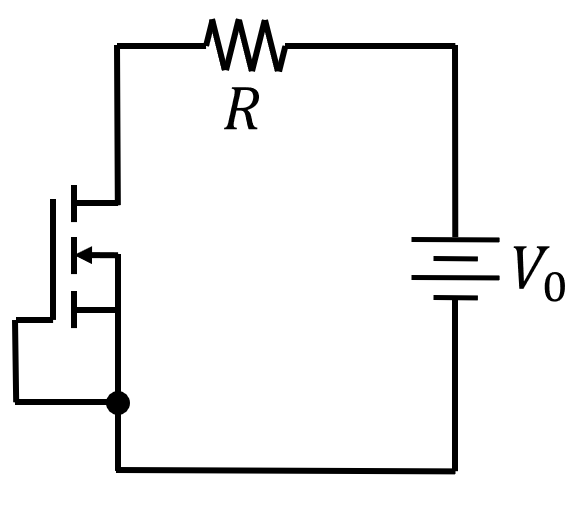
\includegraphics[width=\linewidth]{figures/MOSFET_circuit.png}
    \caption{}
    \label{MOSFET_circuitfig_a}
  \end{subfigure}%
  %\hspace*{\fill}   % maximize separation between the subfigures
  \begin{subfigure}{0.23\textwidth}
    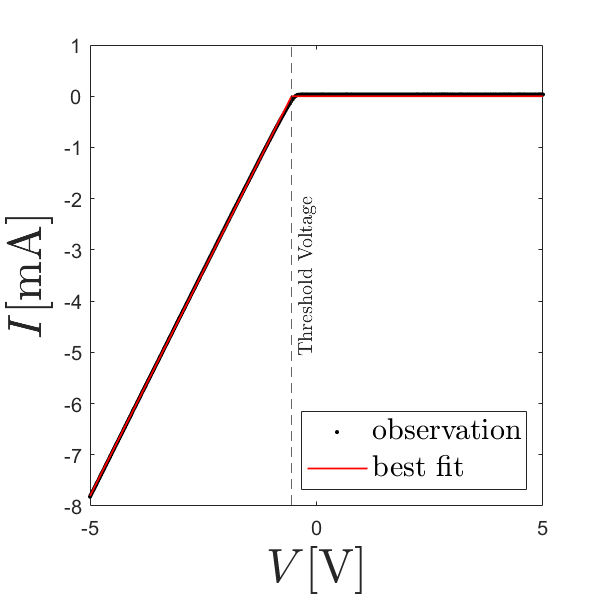
\includegraphics[width=\linewidth]{figures/MOSFETIV.png}
    \caption{}
    \label{MOSFET_circuitfig_b}
  \end{subfigure}

\caption{(a) A schematic setup for testing MOSFET $I-V$ characteristic. (b) Experimental result of MOSFET $I-V$ characteristic. Black dots show experiment data and red line is the best fit to Eq. \ref{MOSFET_eq}. Threshold voltage is denoted as dashed line.} \label{MOSFET_circuitfig}
\end{figure}

In this experiment we used two MOSFETs with gate terminal and source terminal connected each other.
MOSFET is open when the gate--source voltage is higher than the threshold voltage, and current through MOSFET linearly increases as gate--drain voltage increases.
We can characterize this property as 

\begin{equation}
I=\frac{V-V_{\textrm{th}}}{(R+R_{\textrm{MOS}})}\theta(V-V_{\textrm{th}})
\label{MOSFET_eq}
\end{equation}

\noindent where $V_{\textrm{th}}$ is threshold voltage, $R_{\textrm{MOS}}$ is effective resistance of MOSFET, and $\theta(V)$ is Heaviside step function.
To test this $I-V$ characteristic, we set the circuit as Fig. \ref{MOSFET_circuitfig_a}.
We sourced voltage from -5.00V to +5.00V in increments of 0.1V, with a resistor of $R=$560 $\Omega$.
The result is plotted in Fig. \ref{MOSFET_circuitfig_b}, where experimental data is denoted as black dots, best fit to Eq. \ref{MOSFET_eq} as red line, and threshold voltage as dashed line.
Note that the gate--drain voltage is negative when $V_{0}>0$ and vice versa in this setup, so we put $(V-V_{\textrm{th}})\rightarrow-(V-V_{\textrm{th}})$ and $I\rightarrow -I$ into the equation.
Our best fit values are $V_{\textrm{th}}=0.5505\pm0.0015$ V and $R_{\textrm{MOS}}=10.21\pm0.33\>\Omega$.


\section{Derivation of the theoretical $I-V$ Characteristics of the Negative Resistor}

\begin{figure}[!h]
  \centering
  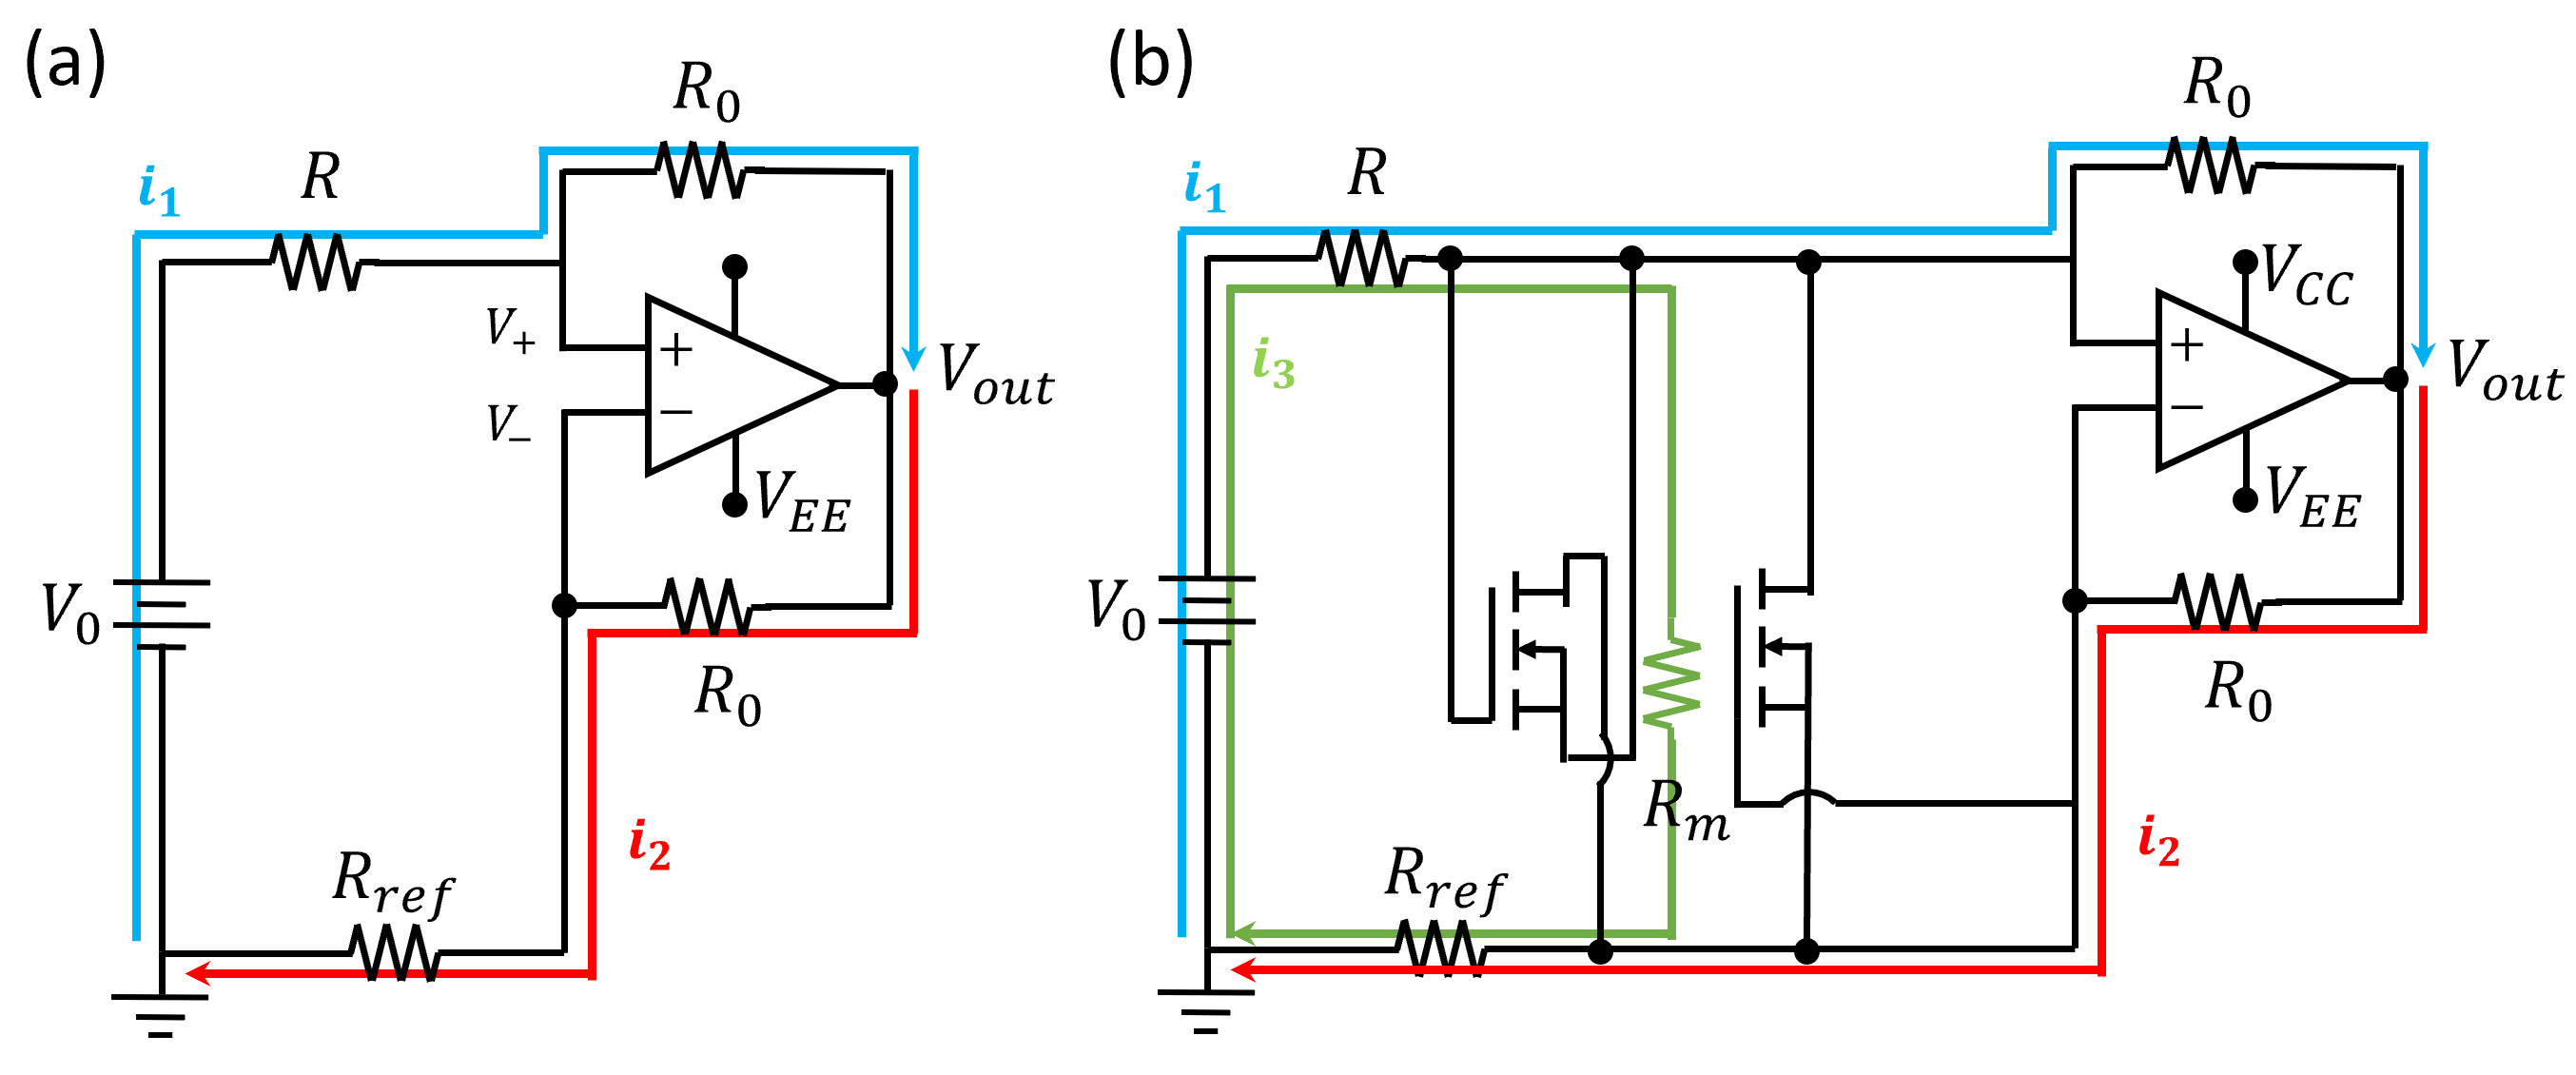
\includegraphics[width=0.45\textwidth]{figures/Appendix2.png}
  \caption{The (a) capacitance and (b) resistance about the normalized deviation of phase difference. }
  \label{fig:OpAmpTheory}
\end{figure}

\subsubsection{\label{opampiv}Op-Amp}
For the negative resistor with only an Op-Amp an ideal op amp is assumed for the theoretical calculation of the unsaturated region. Therefore, the input voltage of the Op-Amps are identical($V_+=V_-$). Using this fact, following Fig.\ref{fig:OpAmpTheory} the following equations are obtained.
\begin{eqnarray}
  V_{in}-Ri_1 = V_+\\
  V_+ -R_0i_1 = V_{out}\\
  V_{out}-R_0i_2=V_-\\
  V_--R_{ref}i_2=0\\
  V_+ = V_-
\end{eqnarray}
By solving these $5$ equations, the following results can be obtained.
\begin{eqnarray}
  V_{out} = \frac{R_{ref}+R_0}{R_{ref}-R}V_{in}\\
  i_1 = -\frac{1}{R_{ref}-R}V_{in}
\end{eqnarray}

\subsubsection{\label{opamp_mosfetiv}Op-Amp and MOSFETs}
The unsaturated region of the negativer resistor using enabling MOSFETs is identical to the unsaturated region of the negative resistor without the MOSFETs, since all of the MOSFETs do not flow current. We derive a theoretical description of the differential resistance slopes for the region where a MOSFET is opened. 

The three currents present after saturation are depicted in Fig. . In the saturated state, the output voltage of the Op-Amp is fixed as $V_{out}-V_{sat}$. Then the following equations can be obtained.


\begin{eqnarray}
  V_{sat} = V_{in}-R(i_1+i_2)-i_1R_0\\
  V_{in} - R(i_1+i_2)-R_mi_2-R_{ref}(i_2+i_3) = 0\\
  V_{sat} -i_3R_0-(i_2+i_3)R_{ref} = 0\\
\end{eqnarray}

When solving the previous equations, a solution we can obtain is the following:
\begin{widetext}
\begin{eqnarray}
  i_1 = \frac{V_{sat}(-R_0R_{ref}-R_0R-R_mR_0-R_mR_{ref})+V_{in}(R_0R_{ref}+R_mR_0+R_mR_{ref})}{R_0^2R_{ref}+R_0^2R+R_mR_0^2+2R_0R_{ref}R+R_mR_0R_{ref}+R_mR_0R+R_mR_{ref}R}\\
  i_2 = \frac{R_0(V_{sat}(-R_{ref}+R)+V_{in}(R_0+R_{ref}))}{R_0^2R_{ref}+R_0^2R+R_mR_0^2+2R_0R_{ref}R+R_mR_0R_{ref}+R_mR_0R+R_mR_{ref}R}\\
  i_3 = \frac{V_{sat}(R_0R_{ref}+R_0R+R_mR_0+R_mR)-V_{in}R_0R_{ref}}{R_0^2R_{ref}+R_0^2R+R_mR_0^2+2R_0R_{ref}R+R_mR_0R_{ref}+R_mR_0R+R_mR_{ref}R}
\end{eqnarray}
\end{widetext}
The current flowing through $R$ is $i_1+i_2$, thus giving the proportional constant to $V_{in}$ as the following:
\begin{widetext}
\begin{equation}
  i_1+i_2 = \frac{R_0R_{ref}+R_0R_m+R_mR_{ref}+R_0^2+R_{ref}R_0}{R_0^2(R_{ref}+R+R_m)+R_0(2R_{ref}R+R_{ref}R_m+R_mR)+R_mR_{ref}R}V_{in} + \text{Intercept}
\end{equation}
\end{widetext}

\bibliographystyle{unsrt}
\bibliography{references}
\end{document}
